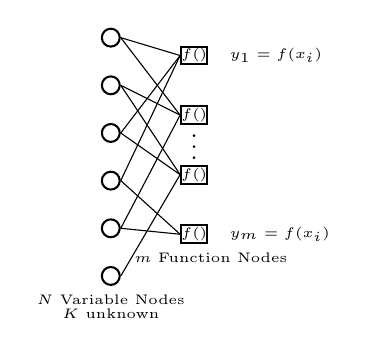
\begin{tikzpicture}
\def\horzgap{7ex}; %Horizontal gap between nodes/levels
\def \gapVN{4ex}; %vertical gap between variable nodes
\def \gapCN{5ex}; %Horizontal gap between check nodes
\def\nodewidth{1.5ex};

\def \textoffs{1ex}; %Offset for writing text east of a node
%\def\nodewidthA{0.05in};
%\def \edgewidth{0.02in};
%\def\ext{0.2in};
`
\def \n{8};
\def\ldeg{2};
\def \m {4};
\def\rdeg{3};

\def\langle{40};%120 degrees/3
\def\langle{20};%120 degrees/6

\tikzstyle{check} = [rectangle, draw, line width=0.75pt, inner sep=0mm, minimum height=\nodewidth, minimum width=\nodewidth]
\tikzstyle{bit} = [circle, draw,line width=0.75pt, inner sep=0mm, minimum size=\nodewidth]

                          
\foreach \vn in {1,...,6}{
 \node[bit] (vn\vn) at (0,-\vn*\gapVN) {};
}


\foreach \cn in {1,...,4}{
\node[check] (cn\cn) at (\horzgap,-0.1*\gapCN-\cn*\gapCN) {\tiny{$f()$}};
}

\path (cn2)++(0,-0.4*\gapCN) node () {\small{$\vdots$}};
\path (cn1.east)++(\textoffs,0) node ()[anchor=west] {\tiny{$y_1=f(x_i)$}};
\path (cn4.east)++(\textoffs,0) node ()[anchor=west] {\tiny{$y_m=f(x_i)$}};

\draw (vn4.east)--(cn4.west);
\draw  (vn5.east)--(cn4.west);

\draw (vn2.east)--(cn3.west);
\draw (vn3.east)--(cn3.west);
\draw  (vn6.east)--(cn3.west);

\draw (vn1.east)--(cn2.west);
\draw (vn2.east)--(cn2.west);
\draw (vn5.east)--(cn2.west);

\draw (vn1.east)--(cn1.west);
\draw (vn3.east)--(cn1.west);
\draw (vn4.east)--(cn1.west);

%\node[text width=1.5cm] () at (0,-6.5*\gapVN){\tiny $N$ Variable Nodes $K$ unknown};
\node[align=left] () at (0,-6.5*\gapVN){\tiny $N$ Variable Nodes};
\node[align=left] () at (0,-6.8*\gapVN){\tiny $K$ unknown};
\node () at (1.2*\horzgap,-4.5*\gapCN){\tiny $m$ Function Nodes};

\end{tikzpicture}